\documentclass[20pt]{beamer}
\usepackage{array} % Used for > in Resources table

% Colours come from colour brewer
\usepackage{xcolor}
\definecolor{b-blue}{HTML}{6baed6}
\definecolor{b-darkgrey}{HTML}{2D2D2D}
\definecolor{b-grey}{HTML}{969696}
\definecolor{b-purple}{HTML}{9e9ac8}
\definecolor{b-green}{HTML}{74c476}
\definecolor{b-pink}{HTML}{e377c2}
\definecolor{b-orange}{HTML}{FD8D3C}

\usepackage{relsize}

\usepackage{fontspec}
\defaultfontfeatures{Mapping=tex-text} % enable -- / --- / `` / ''
\setsansfont[ItalicFont={* Light},BoldItalicFont={* ExtraLight}]{Yanone Kaffeesatz}
\setmonofont[Scale=0.75]{Bitstream Vera Sans Mono}

% Neutralise underscores, since we don't use them apart for in URLs
\catcode`_=12
\begingroup\lccode`~=`_\lowercase{\endgroup\let~\sb}
\mathcode`_="8000

\usepackage{tikz}
\usetikzlibrary{positioning}
\usetikzlibrary{shapes.geometric}
\usetikzlibrary{calc}
% Useful for pictures.
\tikzstyle{nopadding} = [inner sep=0cm]
\tikzstyle{attribution} = [fill=b-darkgrey, anchor=south,
outer sep=0, inner sep=.1ex, font=\relsize{-6}\it,
minimum width=\paperwidth, text width=.95\paperwidth]

\newcommand{\hero}[1]{%
  \begin{tikzpicture}[remember picture, overlay]%
  \node[anchor=west,align=left,font=\Huge\bfseries] (A) at ($(current page.west) + (0.05\paperwidth, .17\paperheight)$) {%
    #1
  };
\end{tikzpicture}}

\newcommand{\herohigh}[1]{%
  \begin{tikzpicture}[remember picture, overlay]%
  \node[anchor=west,align=left,font=\Huge\bfseries] (A) at ($(current page.west) + (0.05\paperwidth, .25\paperheight)$) {%
    #1
  };
\end{tikzpicture}}

\newcommand{\minionhigh}[1]{%
  \begin{tikzpicture}[remember picture, overlay]%
  \node[anchor=west,align=left,font=\Large\bfseries] (A) at ($(current page.west) + (0.05\paperwidth, .25\paperheight)$) {%
    #1
  };
\end{tikzpicture}}

\newcommand{\upperhalf}[1]{%
  \begin{tikzpicture}[remember picture, overlay]%
    \node[anchor=west,font=\normalsize, align=left] at
    ($(current page.west) + (0.05\paperwidth, .25\paperheight)$) {%
      #1
    };
  \end{tikzpicture}
}

\newcommand{\lowerhalf}[1]{%
  \begin{tikzpicture}[remember picture, overlay]%
    \node[anchor=west,font=\normalsize, align=left] at
    ($(current page.west) + (0.05\paperwidth, -.25\paperheight)$) {%
      #1
    };
  \end{tikzpicture}
}

\newcommand{\bottomhalf}[1]{%
  \begin{tikzpicture}[remember picture, overlay]%
    \node[anchor=south west,font=\normalsize, align=left] at
    ($(current page.south west) + (0.05\paperwidth, 0)$) {%
      #1
    };
  \end{tikzpicture}
}

\newcommand{\inthemiddle}[1]{%
  \begin{tikzpicture}[remember picture, overlay]%
    \node at (current page.center) {%
      #1
    };
  \end{tikzpicture}
}

\newcommand{\bottomleft}[1]{%
  \begin{tikzpicture}[remember picture, overlay]%
    \node[anchor=south west, align=left,font=\footnotesize] at (current page.south west) {%
      #1
    };
  \end{tikzpicture}
}

\newcommand{\bottomright}[1]{%
  \begin{tikzpicture}[remember picture, overlay]%
    \node[anchor=south east, align=right,font=\footnotesize] at (current page.south east) {%
      #1
    };
  \end{tikzpicture}
}

\newcommand{\bottomhanging}[1]{%
  \begin{tikzpicture}[remember picture, overlay]%
    \node[anchor=north] at
    ($(current page.center) + (0, .17\paperheight)$) {
      #1
    };
  \end{tikzpicture}
}

\newcommand{\bottomhangingleft}[1]{%
  \begin{tikzpicture}[remember picture, overlay]%
    \node[anchor=north west,align=left] at
    ($(current page.west) + (0.05\paperwidth, .17\paperheight)$) {
      #1
    };
  \end{tikzpicture}
}


\usepackage{fontawesome}
\newfontfamily{\FA}{FontAwesome}
\def\twitter{{\FA \faTwitter}}
\def\heart{{\FA \faHeart}}
\def\tickmark{{\FA \faCheck}}
\def\rarrow{{\FA \relsize{-1}{\faArrowRight}}}
\def\imagetop#1{\vtop{\null\hbox{#1}}}

\newcommand{\hrefp}[2]{\href{#1://#2}{#2}}
\newcommand{\twitterhandle}[1]{\href{https://twitter.com/#1}{@#1}}
\newcommand{\twitterhandlesm}[1]{\relsize{-1}{\color{b-grey}\href{https://twitter.com/#1}{@#1}}}

\begin{document}

% TODO: switch to https://github.com/andreberg/Meslo-Font or with Deja
%   Vu Sans Mono http://9-bits.com/post/123940811/menlo-font-macosx so
%   that it works cross-platform.
% TODO: Simplify snippets to use plain background?

% Enforce colours and styles for beamer:
\setbeamercolor*{palette primary}{fg=white,bg=b-darkgrey}
\setbeamercolor*{titlelike}{parent=palette primary}
\setbeamercolor*{normal text}{parent=palette primary}
\setbeamercolor*{itemize}{parent=palette primary}
\color{white}

\setbeamertemplate{navigation symbols}{}
\setbeamercolor{itemize/enumerate body}{fg=white}
\setbeamercolor{enumerate item}{fg=white}
\setbeamertemplate{itemize item}{\raisebox{.33ex}{\footnotesize\color{white}$\blacktriangleright$}}

\begin{frame} % 1
  \begin{tikzpicture}[remember picture, overlay]
    \node (A) at ($(current page.center) + (0, .17\paperheight)$) {
      \resizebox{.9\paperwidth}{!}{%
        \color{b-blue}\bf reproducible research}
    };
    \node[anchor=north] at (A.south) {
      \color{b-green}\Large (a simple case)
    };
    \color{white}
    \node[anchor=south west] (B) at
    ($(current page.south west) + (0.05\paperwidth, 0.05\paperwidth)$) {
      \color{b-grey}\twitterhandle{phylorich} \& \twitterhandle{mwpennell}
    };
    \node[anchor=south west] at (B.north west) {
      Rich FitzJohn \& Matt Pennell
    };
  \end{tikzpicture}
\end{frame}

\begin{frame} % 5
  \begin{tikzpicture}[remember picture, overlay]
    \node[inner sep=0, outer sep=0] at (current page.center) {
      \includegraphics[height=\paperheight]{pics/how_much_wood}
    };
    \node[anchor=east,align=right,font=\Large\bfseries] (A) at
    ($(current page.east) + (-0.05\paperwidth, .17\paperheight)$) {%
      {\color{black}How many} species are woody?
    };
    \node[attribution] at (current page.south) {
      \color{b-blue}
      \href{http://scienceimage.csiro.au/image/4447/aristyda-grassland-about-30kms-west-of-charters-towers-qld-/}{QLD
        grassland} \color{white} by Willem van Aken\hfill
      \color{b-blue}
      \href{http://scienceimage.csiro.au/image/3829/tropical-rainforest-canopy-near-cairns-qld-/}{QLD
      rainforest} \color{white} by Willem van Aken
    };
  \end{tikzpicture}
\end{frame}

\begin{frame} % 6
  \inthemiddle{%
    \includegraphics<1>[width=.9\paperwidth]{diagrams/diversity_venn0}%
    \includegraphics<2>[width=.9\paperwidth]{diagrams/diversity_venn1}%
    \includegraphics<3>[width=.9\paperwidth]{diagrams/diversity_venn2}}
\end{frame}

\begin{frame} % 7
  \begin{tikzpicture}[remember picture, overlay]
    \node[inner sep=0, outer sep=0] at (current page.center) {
      \includegraphics[height=\paperheight]{pics/taxonomic_structure}
    };
    \node[anchor=east,align=right,font=\Large\bfseries] (A) at
    ($(current page.east) + (-0.18\paperwidth, .4\paperheight)$) {%
      {\color{b-darkgrey}Missing data} has structure
    };
    \node[anchor=south,font=\Large\bfseries,align=center] at
    ($(current page.south) + (-0.25\paperwidth, 0.07\paperheight)$) {
      100\%\\[-.7ex]non-woody
    };
    \node[anchor=south,font=\Large\bfseries,align=center] at
    ($(current page.south) + (0.25\paperwidth, 0.07\paperheight)$) {
      \color{b-darkgrey}100\%\\[-.7ex]\color{b-darkgrey}woody
    };
    \node[attribution] at (current page.south) {
      \color{b-blue}
      \href{http://commons.wikimedia.org/wiki/File:Donkey_orchid_gnangarra_01.jpg}{Donkey
      orchid} \color{white} by Gnangarra\hfill
    \color{b-blue}
    \href{http://scienceimage.csiro.au/image/4015/bark-patterns-on-a-red-river-gum/}{Red
      river gum} \color{white} by Willem van Aken
    };
  \end{tikzpicture}
\end{frame}

\begin{frame} % 8
  \herohigh{Tools we used}
  \begin{tikzpicture}[remember picture, overlay]%
    \node[anchor=west,font=\normalsize, align=left] at
    ($(current page.west) + (0.05\paperwidth, -.18\paperheight)$) {%
      \begin{minipage}{\textwidth}
        \begin{itemize}
        \item {\color{b-orange}\bf knitr}: what are we trying to make work?
        \item {\color{b-purple}\bf git}: I swear it used to work
        \item {\color{b-green}\bf make}: it takes a while to make it work
        \item {\color{b-pink}\bf travis-CI}: will it work elsewhere?
        \item {\color{b-blue}\bf packrat}: will it work later?
        \end{itemize}
      \end{minipage}
    };
  \end{tikzpicture}
\end{frame}

\begin{frame} % 9
  \hero{Literate programming\\[-.7ex]\color{b-orange} knitr}
  \bottomleft{\hrefp{http}{yihui.name/knitr}}
  \lowerhalf{What are we trying to make work?}
  \note{
    Knitr is the poster child of reproducible research in R.

    Before Knitr, we had Sweave that targetted \LaTeX\ as output.
    Knitr mostly targets markdown, and via pandoc you can convert to
    anything you want.

    The idea is really old (Donald Knuth's CWEB)
  }
\end{frame}

\begin{frame} % 13
  \minionhigh{In a nutshell:}
  \bottomhalf{%
    \begin{tabular}{lll}
      \raisebox{3em}{%
        \includegraphics[width=.3\textwidth]{snippets/knitr_source}}&
      \raisebox{1.5em}{%
        \includegraphics[width=.3\textwidth]{snippets/knitr_processed}}&
    \includegraphics[width=.375\textwidth]{snippets/knitr_html}
    \end{tabular}
    }
\end{frame}

\begin{frame} % 18
  \inthemiddle{\includegraphics[height=\paperheight]{pics/draw_an_owl}}  

  \note{Trivial examples are really easy (this is the owl with two
    circles).  There are some really nice features to help with moving
    beyond trivial cases too:

    \begin{itemize}
    \item caching
    \item automatically picking up plots
    \item direct conversion of R tables to Latex/markdown tables
    \item run code without it appearing in the document
    \item have code in the document but don't run it
    \end{itemize}

    but part of the beauty of it is that you don't have to hold a lot in
    your head: it's just really simple and gets out of the way.}
\end{frame}

\begin{frame} % 19
  \herohigh{Barriers to \color{b-orange} knitr}%
  \only<1>{\bottomhanging{\includegraphics[width=.5\paperwidth]{pics/sausage_factory}}}%
  \lowerhalf{
    \only<2>{Encourages overuse of global variables}%
    \only<3>{Re-running analyses because of\\
      changed punctuation gets annoying}%
    \only<4>{Requires really good editor support}
  }
  \only<4>{%
    \bottomleft{\hrefp{http}{rstudio.com}}%
    \bottomright{\includegraphics[width=.15\paperwidth]{pics/rstudio}}%
  }
  \note{
    \begin{itemize}
    \item Basic data munging is just not that interesting to wade
      through
    \item Programs just aren't that enjoyable to read.  I think this
      is better for technical documentation than for the average
      paper.
    \item Encourages using global variables for everything
    \item Rerunning the entire analysis because you changed some
      punctuation in the text is silly.  Getting the caching right is
      hard and it's fragile.
    \item Requires a really good editor to switch between two
      different programming modes.  Rstudio supports this though.
    \end{itemize}
  }
\end{frame}

\begin{frame} % 20
  \herohigh{Prospects for \color{b-orange} knitr}
  \lowerhalf{
    \only<1>{{\color{b-pink}\bf Amazing} for supporting materials,\\
      manuals, technical documentation\\
      \small \textbf{Examples}: \color{b-grey}\hrefp{https}{github.com/richfitz/reproducibility-2014/wiki}}%
    \only<2>{Generate {\color{b-orange}knitr} files from plain R source:\\
      \qquad\texttt{knitr::spin}\\
      \qquad sowsear:
      \small\color{b-grey}\hrefp{http}{github.com/richfitz/sowsear}}%
    \only<3>{The {\color{b-blue}principle} holds elsewhere:\\
      \textbf{\color{b-green}Output} should be regeneratable from 
      \textbf{\color{b-green}input}}%
  }
  \note{
    \begin{itemize}
    \item This field is moving really quickly, and the tools are
      getting better all the time.
    \item Amazing for supporting materials, especially for technical
      papers.  Saves time for authors, guaranteed correct output for
      readers.
    \item Things to target knitr: sowsear and knitr's \code{spin}
      (give an example here)
    \item The \emph{principle} carries over to non-knitr work though:
      the figures should always be regeneratable from the code.  You
      don't need fancy formatting for that to happen though, just a
      sensible layout of a project and some care.
    \end{itemize}
  }
\end{frame}

% Make the point that simply docuementing where things come from is
% basically good enough
%
% http://karthik.github.io/useR2014/#data_life_cycle
% http://theconversation.com/the-reinhart-rogoff-error-or-how-not-to-excel-at-economics-13646
%
\begin{frame} % 33
  \hero{Workflows\\[-.7ex]\color{b-green} make}
  \lowerhalf{It takes a while to make it work}
\end{frame}

\begin{frame} % 34
  \herohigh{Our workflow}
  \bottomhalf{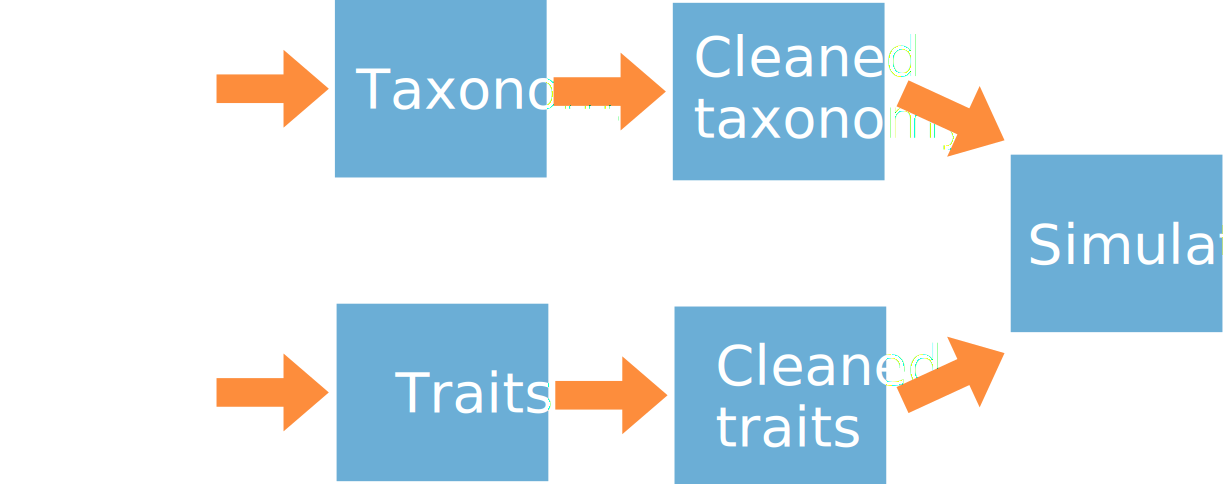
\includegraphics[width=.85\paperwidth]{diagrams/make_workflow}}
  \note{
    Analyses have a chain of dependencies.  Ours was:

    \begin{enumerate}
    \item Download data
    \item Preprocess data to clean it up
    \item Run the simulations
    \end{enumerate}
  }
\end{frame}

\begin{frame} % 35 -- matt has drop
  \only<1>{\minionhigh{Download data}}
  \only<2>{\minionhigh{Rcurl, API access}}
  \only<3>{\minionhigh{Makefile}}
  \bottomhalf{%
    \includegraphics<3>[height=4ex]{snippets/make_download1}\\[1ex]
    \includegraphics[width=.85\paperwidth]{diagrams/make_workflow_download1}}
\end{frame}

\begin{frame} % 36
  \only<1>{\minionhigh{Process data}}%
  \only<2>{\minionhigh{Makefile}}%
  \bottomhalf{%
    \includegraphics<2>[height=4ex]{snippets/make_process1}\\[1ex]
    \includegraphics[width=.85\paperwidth]{diagrams/make_workflow_process1}}
\end{frame}

\begin{frame} % 37 -- matt has drop
  \only<1>{\minionhigh{Run the actual science bit}}
  \only<2>{\minionhigh{Makefile}}
  \bottomhalf{%
    \includegraphics<2>[height=5ex]{snippets/make_simulation}\\[1ex]
    \includegraphics[width=.85\paperwidth]{diagrams/make_workflow_simulation}}
\end{frame}

\begin{frame} % 38 -- matt has drop
  \minionhigh{{\color{b-green}make:}\\[-.4ex]Self-documenting workflow}
  \bottomhalf{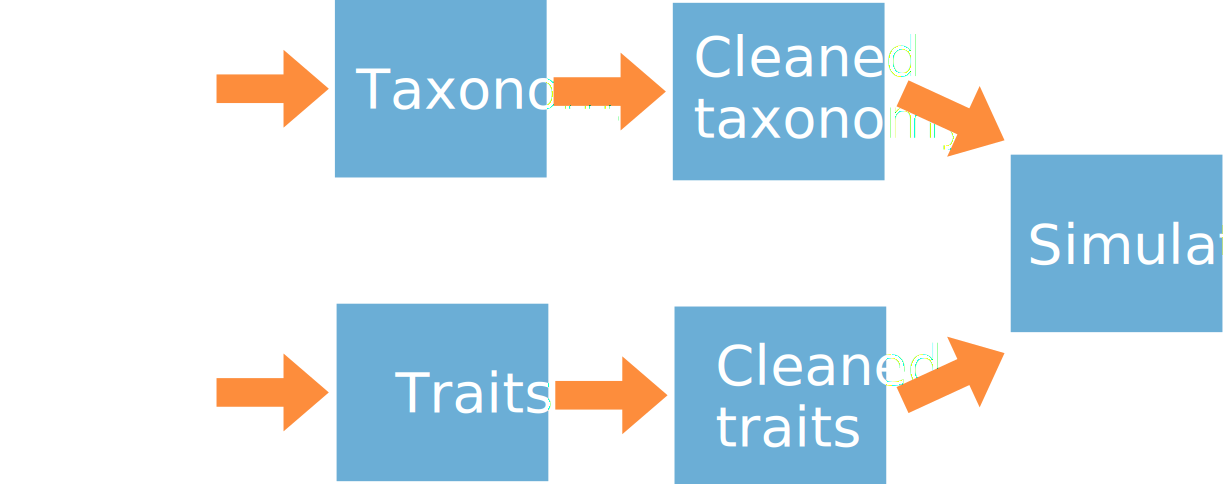
\includegraphics[width=.85\paperwidth]{diagrams/make_workflow}}
  \note{
    The good:
    \begin{itemize}
    \item we end up with a nice definition of "upstream" sources.
    \item once in place, things run nicely, and have a good chance of
      working elsewhere
    \item a bit of thought helps to separate "inputs" (things that you
      provide) and generated content that you should be able to blow
      away.  This is really important.
    \end{itemize}
  }
\end{frame}

\begin{frame} % 39 -- matt has drop
  \hero{Workflows\\[-.7ex]\color{b-green} make}
  \lowerhalf{Why doesn\kern-1pt't everyone use this all the time?}
\end{frame}

\begin{frame} % 40
  \herohigh{Barriers to \color{b-green} make}
  \lowerhalf{
    \only<1>{{\color{b-pink}\textbf{Lots}} of traps}%
    \only<2>{Command-line only, arcane tool\\%
    Comes in several incompatible flavours}%
    \only<3>{Currently looking for a\\modern, accessible replacement}%
  }
  \note{
    The bad:
    \begin{itemize}
    \item put up a picture of our makefile
    \item Pretty arcane
    \item basically needs replacing with something pleasant, R-ish, and
      enjoyable to use
    \item knitr's caching can do this to some degree, but I find it fragile.
    \item where I hope we can go is a declarative style ``this function
      depends on these things and produces this thing'' that can be used
      to stick together complex analyses.
    \item New web package management things (e.g. bower.io) might help
      here.
    \item Perhaps show where we're heading with model adequacy?
    \item otherwise I consider this one unsolved for current non-computer
      scientists.
    \end{itemize}
  }
\end{frame}

% TODO: Add 2 new slides for maker (e.g., model adequacy)

\begin{frame} % 41
  \hero{Automated testing\\[-.4ex]\color{b-pink} travis-CI}
  \lowerhalf{Will it work elsewhere?}
  \bottomleft{\hrefp{http}{travis-ci.org}}
  \note{
    Getting into extra-for-experts territory here

    Basic workflow:

    \begin{enumerate}
    \item Make changes
    \item Check things look OK locally
    \item Push to github
    \item Travis spins up (show a few snippets from the logs)
    \item If there's a problem you get an email (ideally show how this
      works with the link in the email, the changeset, etc).
    \end{enumerate}

    The good:

    I think that this is the future.  If we'd been using this from the
    beginning, we'd have noticed lots of problems that affected us
    later.

    Because you find out as soon as things break, you only have to
    look at a small set of changes.  If you're regularly breaking one
    thing you know where you need to put your time.

    You can collect the output from each run and store them somewhere
    - can turn this into a virtual lab notebook!

    The bad:

    \begin{itemize}
    \item not a perfect fit to research
    \item open source public projects only
    \item not going to work with sensitive data
    \item not going to work with long running jobs
    \item what if your research requires running on a cluster for a month?
    \end{itemize}

    Prospects:

    CI platforms focussed on research probably not far away.
    Several self-hosted solutions that institutions could easily set up
    if there is interest
    \begin{itemize}
    \item Atlassian Bamboo CI (Sydney)
    \item Jenkins
    \item Drone
    \end{itemize}
    Pay for a hosted solution, host on digital ocean, etc.
  }
\end{frame}

\begin{frame} % 42
  \minionhigh{\LARGE{\color{b-pink} CI} = \color{b-blue}Continuous Integration}
  \lowerhalf{
    \begin{minipage}{\textwidth}
      \begin{enumerate}
      \item Commit changes
      \item \only<1>{Make sure nothing breaks}%
        \only<2>{\color{b-blue}Push to GitHub\phantom{g}}
      \end{enumerate}
    \end{minipage}
  }
  \note{}
\end{frame}

\begin{frame} % 43
  \minionhigh{%
    \only<1>{Spins up virtual machine\ldots}%
    \only<2>{\ldots installs dependencies\ldots}%
    \only<3>{\ldots downloads and processes data\ldots}%
    \only<4>{\ldots runs \color{b-orange}knitr\phantom{p}\ldots}%
    \only<5>{\ldots \& compiles manuscript.}}
  \bottomhanging{%
    \includegraphics<1>[width=\paperwidth]{shots/travis_log_1_spinup}%
    \includegraphics<2>[width=\paperwidth]{shots/travis_log_2_deps}%
    \includegraphics<3>[width=\paperwidth]{shots/travis_log_3_process}%
    \includegraphics<4>[width=\paperwidth]{shots/travis_log_4_knitr}%
    \includegraphics<5>[width=\paperwidth]{shots/travis_log_5_ms}%
  }
\end{frame}

\begin{frame} % 48
  \herohigh{Barriers to \color{b-pink} travis-CI}
  \lowerhalf{%
    \only<1>{Project must \textbf{\color{b-green}already be reproducible}}%
    \only<2>{Only for open source, or pay}%
    \only<3>{Ill-suited for long running jobs, sensitive data}%
  }
  \note{
    I think that this is the future though.  If we had used this from
    the beginning, our project would have hit fewer hurdles later.
    \begin{itemize}
    \item CI platforms focussed on research probably not far away.
    \item Several self-hosted solutions that institutions could easily
      set up: Atlassian Bamboo, Jenkins, possibly Drone.  Or pay for a
      hosted solution on Amazon, Digital Ocean.
    \end{itemize}
  }
\end{frame}

% 6. Package versioning (2 new slides)
%
% TODO: Rather than focus on packrat, just highlight general issues and possible options (packrat, docker etc.)
\begin{frame} % 49
  \hero{Dependencies\\[-.7ex]\color{b-blue} packrat}
  \bottomleft{\hrefp{http}{rstudio.github.io/packrat}}
  \lowerhalf{Will it work later?}
  \bottomright{See also\\[-.2ex]\href{https://github.com/opower/rbundler}{\color{b-blue}\small rbundler}}
\end{frame}

\begin{frame} % 56
  \hero{{\color{b-green}100\%}\\[-.7ex]reproducible}
  \lowerhalf{%
    \only<2>{\color{b-blue}
      \begin{minipage}{1.0\linewidth}\tt\footnotesize\raggedright
        git clone https://github.com/richfitz/wood/\\
        cd wood\\
        make deps all
      \end{minipage}
      \\[1em]
      \scriptsize\color{b-grey}\ldots provided you have C,
      C++ \& Fortran compilers, make, GNU scientific library, LaTeX.
    }%
    \only<3>{Probably unrealistic at the moment}}
\end{frame}

\begin{frame} % 57
  \hero{{\color{b-green}Partially}\\[-.7ex]reproducible}
  \lowerhalf{
    \only<1>{It\kern-.5pt's not just good --- it\kern-.5pt's good enough}%
    \only<2>{Good faith effort at documenting requirements\\
      makes it \textbf{\color{b-blue}much} easier to pick up}%
  }
\end{frame}

\end{document}

%%% Local Variables:
%%% mode: latex
%%% TeX-PDF-mode: t
%%% TeX-engine: xetex
%%% End:
